\documentclass{article}
\linespread{1.3}
\usepackage[margin=50pt]{geometry}
\usepackage{amsmath, amsthm, amssymb, amsthm, tikz, fancyhdr, graphicx}
\pagestyle{fancy}
\renewcommand{\headrulewidth}{0pt}
\newcommand{\changefont}{\fontsize{15}{15}\selectfont}

\fancypagestyle{firstpageheader}
{
  \fancyhead[R]{\changefont Michael Huang \\ CFRM 420 \\ Homework 1}
}

\begin{document}

\thispagestyle{firstpageheader}

\section*{1.}
{\Large 

\subsection*{(a)}

To calculate the daily arithmetic returns, we take the adjusted stock prices for each day $n$ and simply calculate the daily returns like so: \\
$R(t_{n-1}, t_n) = \frac{{P_t}_n - P_t_{n-1}}{{P_t}_{n-1}}$ \\
Which we then plot.

\begin{figure}[h]
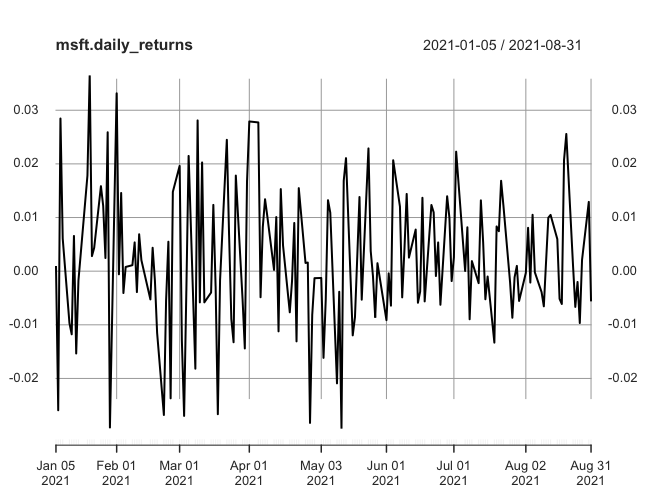
\includegraphics[width=500pt]{hw1_1a.png}}
\centering
\end{figure}

\subsection*{(b)}

To calculate the monthly log returns, we take each time period $n$'s data and evaluate like so: \\
$r(t_{n-1}, t_n) = \text{log}\frac{{P_t}_{n}}{{P_t}_{n-1}}$ \\
which evaluated to the following results: \\

\begin{tabular}{|c|c|}
	\hline
	\textbf{Month} & \textbf{Return} \\
	\hline
	Feb 2021 & 0.004109548 \\
	\hline
	Mar 2021 & 0.014482745 \\
	\hline
	Apr 2021 & 0.067286307 \\
	\hline
	May 2021 & -0.007656559 \\
	\hline
	Jun 2021 & 0.081569730 \\
	\hline
	Jul 2021 & 0.050423540 \\
	\hline
	Aug 2021 & 0.059768866 \\
	\hline
\end{tabular}

}

\section*{2.}
{\Large

%\begin{verbatim}
%  Text enclosed inside \texttt{verbatim}
%  environment 
%  is printed directly 
%  and all \LaTeX{} commands are ignored.
%\end{verbatim}

%\framebox[1.1\width]{\textbf{answer}}

We first calculate the change in price over that time period. We have the prices as follows on each date: \\

\begin{tabular}{|c|c|c|}
	\hline
	\textbf{Date} & \textbf{MSFT.Adjusted} & \textbf{AAPL.Adjusted} \\
	\hline
	2021-01-04 & 216.2754 & 128.8048 \\
	\hline
	2021-05-03 & 250.7996 & 132.1173 \\
	\hline
	2021-08-31 & 301.8800 & 151.8300 \\
	\hline
\end{tabular} \\ \\
We can arbitrarily set our starting portfolio to 1000 for ease of calculation, and see that we start with \\ 
$ 0.6 \cdot 1000 \div 217.2754 = $ 2.774241 MSFT and $ 0.4 \cdot 1000 \div 128.8048 = $ 3.105474 AAPL. \\
which then becomes \\
$ 2.77421 \cdot 250.77996 + 3.105474 \cdot 132.1173 = $ 1106.065,
our new portfolio value which we now need to rebalance. We can recalculate our share counts to be \\
$ 0.4 \cdot 1106.065 \div 250.7996 = $ 1.764062 MSFT and $0.6 \cdot 1106.065 \div 132.1173 = $ 5.023107 AAPL. \\
We then calculate the final value at the end date: \\
$1.76402 \cdot 301.8800 + 5.023107 \cdot 151.8300 = $ 1295.193 \\ \\
Taking this final value into account, we can calculate final arithmetic and logarithmic returns: \\
Arithmetic: $\frac{1295.193 - 1000}{1000} = \framebox[1.1\width]{\textbf{0.2951933}}
$ \\
Logarithmic: $\text{log}\frac{1295.193}{1000} = \framebox[1.1\width]{\textbf{0.2586600}}$

}

\section*{3.}
{\Large 
In the arithmetic return case, we can directly compare by calculating the overall change in value. In the first case, we would have $100 * 1.2 = 120$ percent of the original value after the first month, and then $120 * 0.8 = 96$ percent of the original value after the second month, so the total return would be $-0.04$. We can calculate the return in the same way for the second case. We would have $100 * 0.8 = 80$ percent of the original value after the first month, and then $80 * 1.2 = 96$ percent of the original value after the second month. We see that yet again, we have a total return of $-0.04$, so we can see that in the arithmetic return case, \framebox[1.1\width]{\textbf{the situations are equal.}} \\ \\
In the logarithmic return case, we can calculate the total logarithmic return across the multiple months by simply summing up the logarithmic returns of each month. \\
Doing this in the first case, we find that the logarithmic return is $0.2 + -0.2 = 0$. \\
Doing this in the second case, we find that the logarithmic return is $-0.2 + 0.2 = 0$. \\
We can therefore see that in the logarithmic case as well, \framebox[1.1\width]{\textbf{the situations are equal.}}



%wtf is this
}

\end{document}